\documentclass{beamer}
\usetheme{Copenhagen}
\usecolortheme{beaver}
\setbeamercolor{itemize item}{fg=darkred!80!black}

% PACKAGE IMPORTS
\usepackage[utf8]{inputenc}
\usepackage{tikz}
\usepackage{subcaption}
\usepackage{minted}
\usepackage[normalem]{ulem} % for striking out text with \sout
% END PACKAGE IMPORTS

% TITLE MATTER
\makeatother
\author{Julian}
\title{Webautomation mit Selenium}
\subtitle{Wie man einen Platz im Hochschulsport bekommt}
\institute{Linx AG Blitztalk}
\date{\today}
% END TITLE MATTER

% DEFINITIONS
\newcommand{\smiley}{\tikz[baseline=-0.75ex,black]{
		\draw circle (2mm);
		\node[fill,circle,inner sep=0.5pt] (left eye) at (135:0.8mm) {};
		\node[fill,circle,inner sep=0.5pt] (right eye) at (45:0.8mm) {};
		\draw (-145:0.9mm) arc (-120:-60:1.5mm);
	}
}
% END DEFINITIONS

% PAGE NUMBERING
\expandafter\def\expandafter\insertshorttitle\expandafter{%
	\insertshorttitle\hfill%
	\insertframenumber\,/\,\inserttotalframenumber}
% END PAGE NUMBERING

\begin{document}
	\beamertemplatenavigationsymbolsempty % turn of navigation bar
	\maketitle
	
	
	% TABLE OF CONTENTS
	\begin{frame}
	\frametitle{Layout}
	\tableofcontents
	\end{frame}
	
	\section{Motivation}
	\begin{frame}
	\frametitle{warum?}
	Die Hochschulsport Buchung ist ein Krampf:
	\begin{itemize}
		\item Überlastete Server (weil mehrere Buchungstermine zur gleichen Zeit)
		\item First come first serve Prinzip ...
	\end{itemize}
	\end{frame}
	
	\begin{frame}
	\frametitle{Wie kann man sich helfen?}
	\begin{itemize}
		\item Credentials speichern hilft! (siehe spätere Abbildung)
		\item Maus / Keyboard Makros
		\item EIN SKRIPT!
	\end{itemize}
	\end{frame}

	\section{Die Buchungsseite}
	\begin{frame}
	\frametitle{Wie läuft die Buchung ab?}
	\begin{enumerate}
		\item Kurs der Wahl finden auf der Auswahlseite
		\item Auf der Seite mit Kursbeschreibung den Buchungs-Link finden
		\item Persönliche Daten eingeben
		\item Ein mal bestätigen
		\item Pdf mit Buchungsbestätigung runterladen
	\end{enumerate}
	\end{frame}
	
	\begin{frame}
	\frametitle{Kursauswahl}
	\begin{figure}
		\begin{subfigure}{0.35\textwidth}
			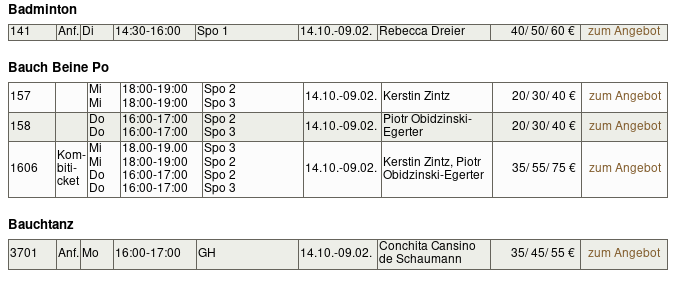
\includegraphics[width=\textwidth]{figures/screenshot_kursliste.png}
			\subcaption{Kursliste}	
		\end{subfigure}
		\begin{subfigure}{0.35\textwidth}
			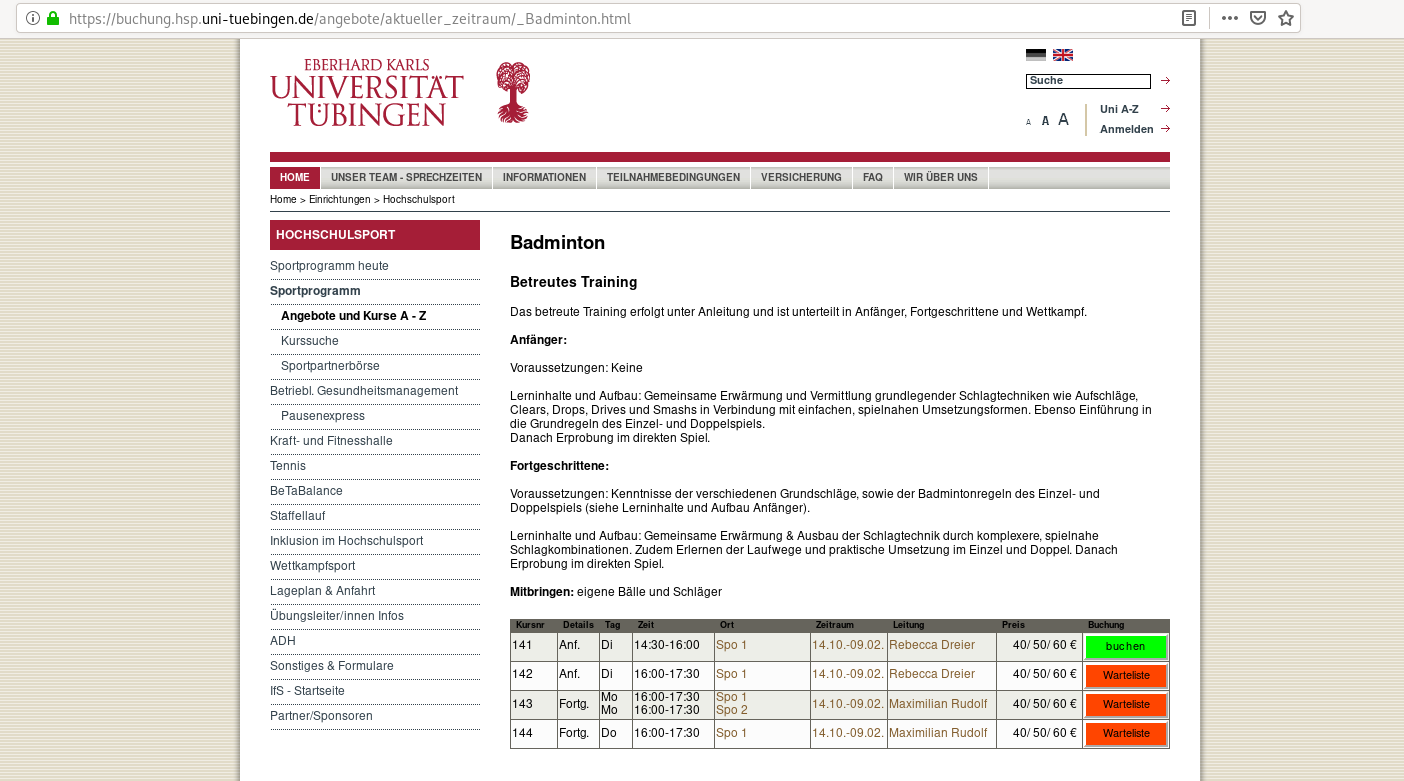
\includegraphics[width=\textwidth]{figures/screenshot_kurs.png}	
			\subcaption{Kursdetailseite}
		\end{subfigure}	
	\end{figure}
	\end{frame}
	
	\begin{frame}
	\frametitle{Kursbuchung}
	\begin{figure}
		\begin{subfigure}{0.32\textwidth}
			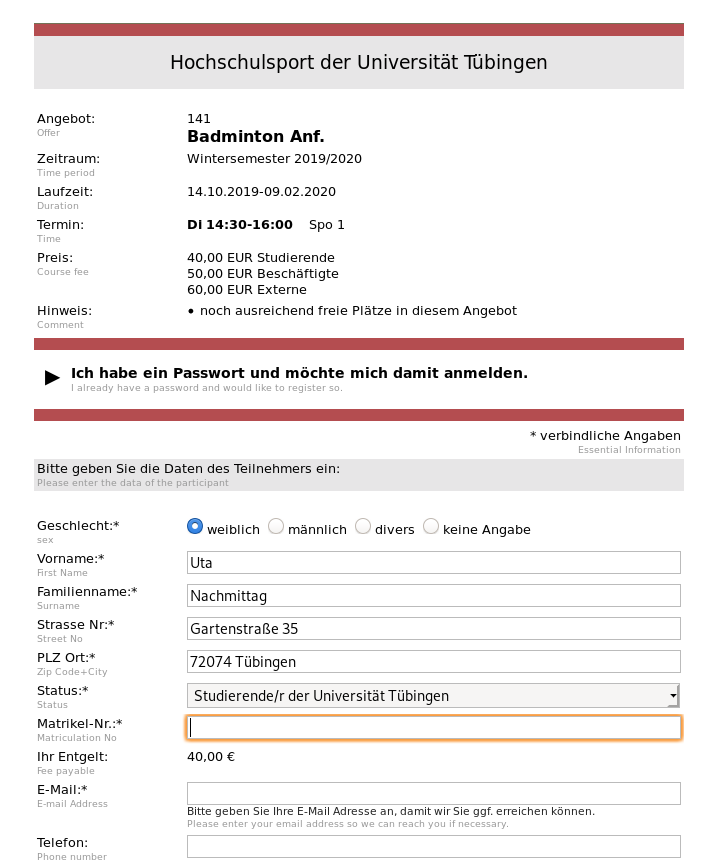
\includegraphics[width=\textwidth]{figures/screenshot_bookingseite.png}
			\subcaption{Dateneingabe}	
		\end{subfigure}
		\begin{subfigure}{0.32\textwidth}
			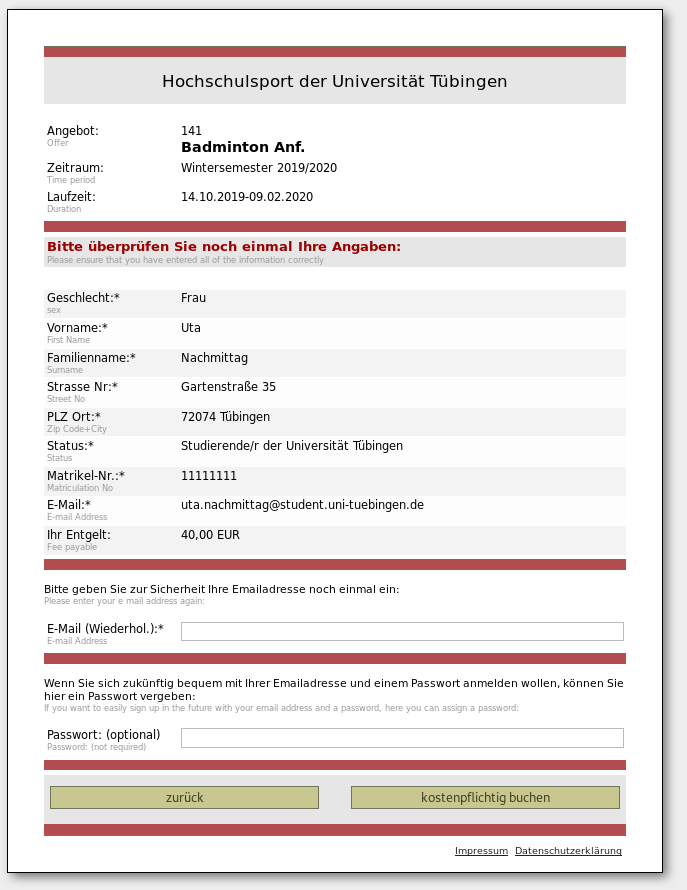
\includegraphics[width=\textwidth]{figures/screenshot_bestaetigung.png}	
			\subcaption{Bestätigung}
		\end{subfigure}	
		\begin{subfigure}{0.32\textwidth}
			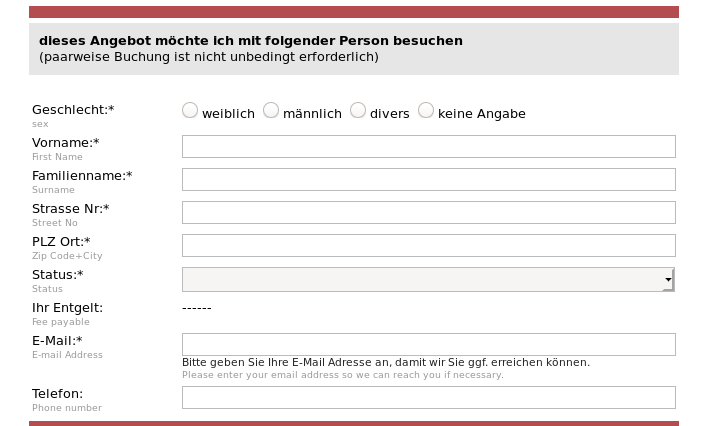
\includegraphics[width=\textwidth]{figures/screenshot_issue3.png}	
			\subcaption{Manchmal mit extra Feld für Partner ...}
		\end{subfigure}	
	\end{figure}
	\end{frame}
	
	\begin{frame}
	\frametitle{Kursbuchung: HTML Formulare}
	\begin{figure}
		\begin{subfigure}{0.8\textwidth}
			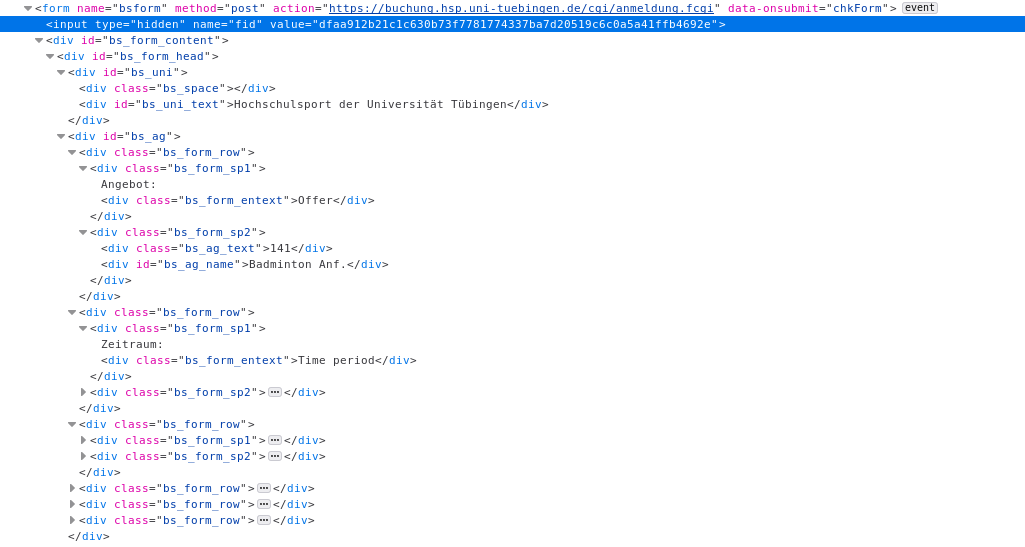
\includegraphics[width=\textwidth]{figures/screenshot_booking_code.png}
			\subcaption{Ein Teil vom Buchungs HTML-Formular (blau markiert eine Session ID)}	
		\end{subfigure}
	\end{figure}
	\end{frame}
	
	
	\begin{frame}
	\frametitle{Security by Obstruction}
	\begin{figure}
		\begin{subfigure}{0.8\textwidth}
			
\includegraphics[width=\textwidth]{figures/screenshot_weird.png}
			\subcaption{.. Im Buchungsformular}	
		\end{subfigure}
	\begin{subfigure}{0.8\textwidth}
		
\includegraphics[width=\textwidth]{figures/screenshut_weird2.png}
		\subcaption{.. Im Bestätigungsformular}	
	\end{subfigure}
	\end{figure}
	\end{frame}
	
	\section{HSP}
	\begin{frame}
		\frametitle{Das Skript: Erste Version (Sommer 2018)}
		Herangehensweise:
		\begin{itemize}
			\item Http Formulare analysiert
			\item Kursseiten, Formularnamen und Session-IDs mit BeautifulSoup4 finden
			\item Mit dem Python Modul requests Session managen, Formulare abschicken (POST Requests ...)
		\end{itemize}
	\end{frame}
	
	\begin{frame}
		\frametitle{Das Skript: Erste Version (Sommer 2018)}
		Herangehensweise:
		\begin{itemize}
			\item Http Formulare analysiert
			\item Kursseiten, Formularnamen und Session-IDs mit BeautifulSoup4 finden
			\item Mit dem Python Modul requests session managen, Formulare abschicken (POST Requests ...)
		\end{itemize}
		
		\vspace{2em}
		{\centering \Large \textbf{Problem: JavaScript}}
	\end{frame}
	
	\begin{frame}
		\frametitle{Das Skript: Zweite Version (Sommer 2019)}
		Nach langer Pause eine neues Vorgehen:
		\begin{itemize}
			\item Kontrolliere Headless Session eines Mozilla Firefox oder Chrome Browsers mit Selenium
			\item Imitiere Nutzer Eingaben
			\item JavaScript, Cookies, Sessions, ... Kein Problem mehr!
		\end{itemize}
	\end{frame}

	\begin{frame}
	\centering
	{\Huge DEMO} 
	
	\vspace{2em}
	
	\url{https://github.com/JulianFlesch/hsp}
	\end{frame}
	
	\begin{frame}
	\frametitle{Andere Lösungen}
	\begin{itemize}
		\item Browser Plugin in JavaScript, das die gleichen Eingaben simuliert
		\item \sout{Wie beim Ansatz von 2018, aber mit der JavaScript Engine phantomjs} \textbf{(Support discontinued)}
	\end{itemize}
	\end{frame}

	\section{Selenium}
	\begin{frame}
	\frametitle{Selenium}
	Hier kommt bald ein kleines Intro ;) 
	\end{frame}

	\begin{frame}
	\centering
	{\Huge Danke fürs Zuhören!} 
	\end{frame}
\end{document}